\revise{This paper mentions several specialized terms that are fundamental to understanding and analyzing the reasoning mechanisms of LLMs. These terms are organized into two categories: conceptual frameworks, which provide theoretical abstractions for modeling LLM reasoning, and empirical analysis methods, which offer practical tools for experimentally probing and validating these frameworks. Below, we provide explanations for these key terms.}

\subsubsection*{\revise{Conceptual frameworks}}
\paragraph{Circuits} Circuits are abstractions of the reasoning logic in deep models. The model $\mathcal{M}$ is viewed as a computational graph. There are two main approaches to modeling circuits. One approach treats the features in the latent space of $\mathcal{M}$ as nodes and the transitions between features as edges.\citep{OldCircuit_20_distill_OpenAI,CausalAbstract_21_NIPS_Stanford} The other approach views different components of $\mathcal{M}$, such as attention heads and neurons, as nodes; and the interactions between these components, such as residual connections, as edges.\citep{IOI_23_ICLR_Redwood} A circuit is a subgraph of $\mathcal{M}$. \revise{Researchers have discovered many important circuits, such as the Bias Circuit,\citep{GenderBias_20_NIPS_Salesforce} Knowledge Circuit,\citep{KnowledgeCircuit_24_arXiv_ZJU} and so on.}

\paragraph{Residual Stream} \revise{As shown in Figure~\ref{fig:ResidualStream}, each row in the figure can be viewed as a residual stream.} The residual stream after layer $\ell$ is the sum of the embedding and the outputs of all layers up to layer $\ell$, serving as the input to layer $\ell+1$. \citet{MathFrame_21_TCT_Anthropic} conceptualized the residual stream as a shared bandwidth through which information can flow. \revise{Different layers (or tokens) utilize this shared bandwidth, with lower layers (or previous tokens) writing information and higher layers (or subsequent tokens) reading it.}

\paragraph{\revise{QK Matrix \& OV Matrix}} \revise{We expand Equation~\ref{equ:attention} into Equation~\ref{equ:QKOV}. According to the study by \citet{MathFrame_21_TCT_Anthropic}, $\mathbf{W_Q}_{\ell}^h  \mathbf{W_K}_{\ell}^{h^\top}$ is referred to as the QK matrix (QK circuit), while $\mathbf{W_V}_{\ell}^h \mathbf{O}_{\ell}^h$ is referred to as the OV matrix (OV circuit). Specifically, the QK matrix enables the computation of attention scores between the $N$ tokens in $\mathbf{X}_{\ell, 0}$, thereby facilitating the reading of information from certain residual streams. Meanwhile, the OV matrix is responsible for writing the processed information back into the corresponding residual streams.}
\vspace{1.2em}
\revise{
\begin{equation}
\label{equ:QKOV}
\begin{aligned}
\operatorname{Attn}_{\ell}^h\left(\mathbf{X}_{\ell, 0}\right) 
&= \operatorname{softmax}\left(\left(\eqnmarkbox[mypurple]{QueryVector}{\mathbf{X}_{\ell, 0} \cdot \mathbf{W_Q}_{\ell}^h}\right) \cdot \left(\eqnmarkbox[mygreen]{KeyVector}{\mathbf{X}_{\ell, 0} \cdot \mathbf{W_K}_{\ell}^h}\right)\right)^\top \cdot \left(\eqnmarkbox[myblue]{ValueVector}{\mathbf{X}_{\ell, 0} \cdot \mathbf{W_V}_{\ell}^h}\right) \cdot \mathbf{O}_{\ell}^h\\
&= \operatorname{softmax}\left(\mathbf{X}_{\ell, 0} \cdot \eqnmarkbox[dark_red_drawio]{QKMatrix}{\mathbf{W_Q}_{\ell}^h  \mathbf{W_K}_{\ell}^{h^\top}} \cdot \mathbf{X}_{\ell, 0}^{\top} \right) \cdot \mathbf{X}_{\ell, 0} \cdot \eqnmarkbox[mygrey]{OVMatrix}{\mathbf{W_V}_{\ell}^h \mathbf{O}_{\ell}^h}
\annotate{above, left, label below}{QueryVector}{Query Vectors' Matrix}
\annotate{above, label below}{KeyVector}{Key Vectors' Matrix}
\annotate{above, label below}{ValueVector}{Value Vectors' Matrix}
\annotate[yshift=-0.5em]{below, label above}{QKMatrix}{QK Matrix}
\annotate[yshift=-0.5em]{below, label above}{OVMatrix}{OV Matrix}
\end{aligned}
\end{equation}
}

\subsubsection*{\revise{Empirical analysis methods}}
\begin{figure}[htbp]
    \centering
    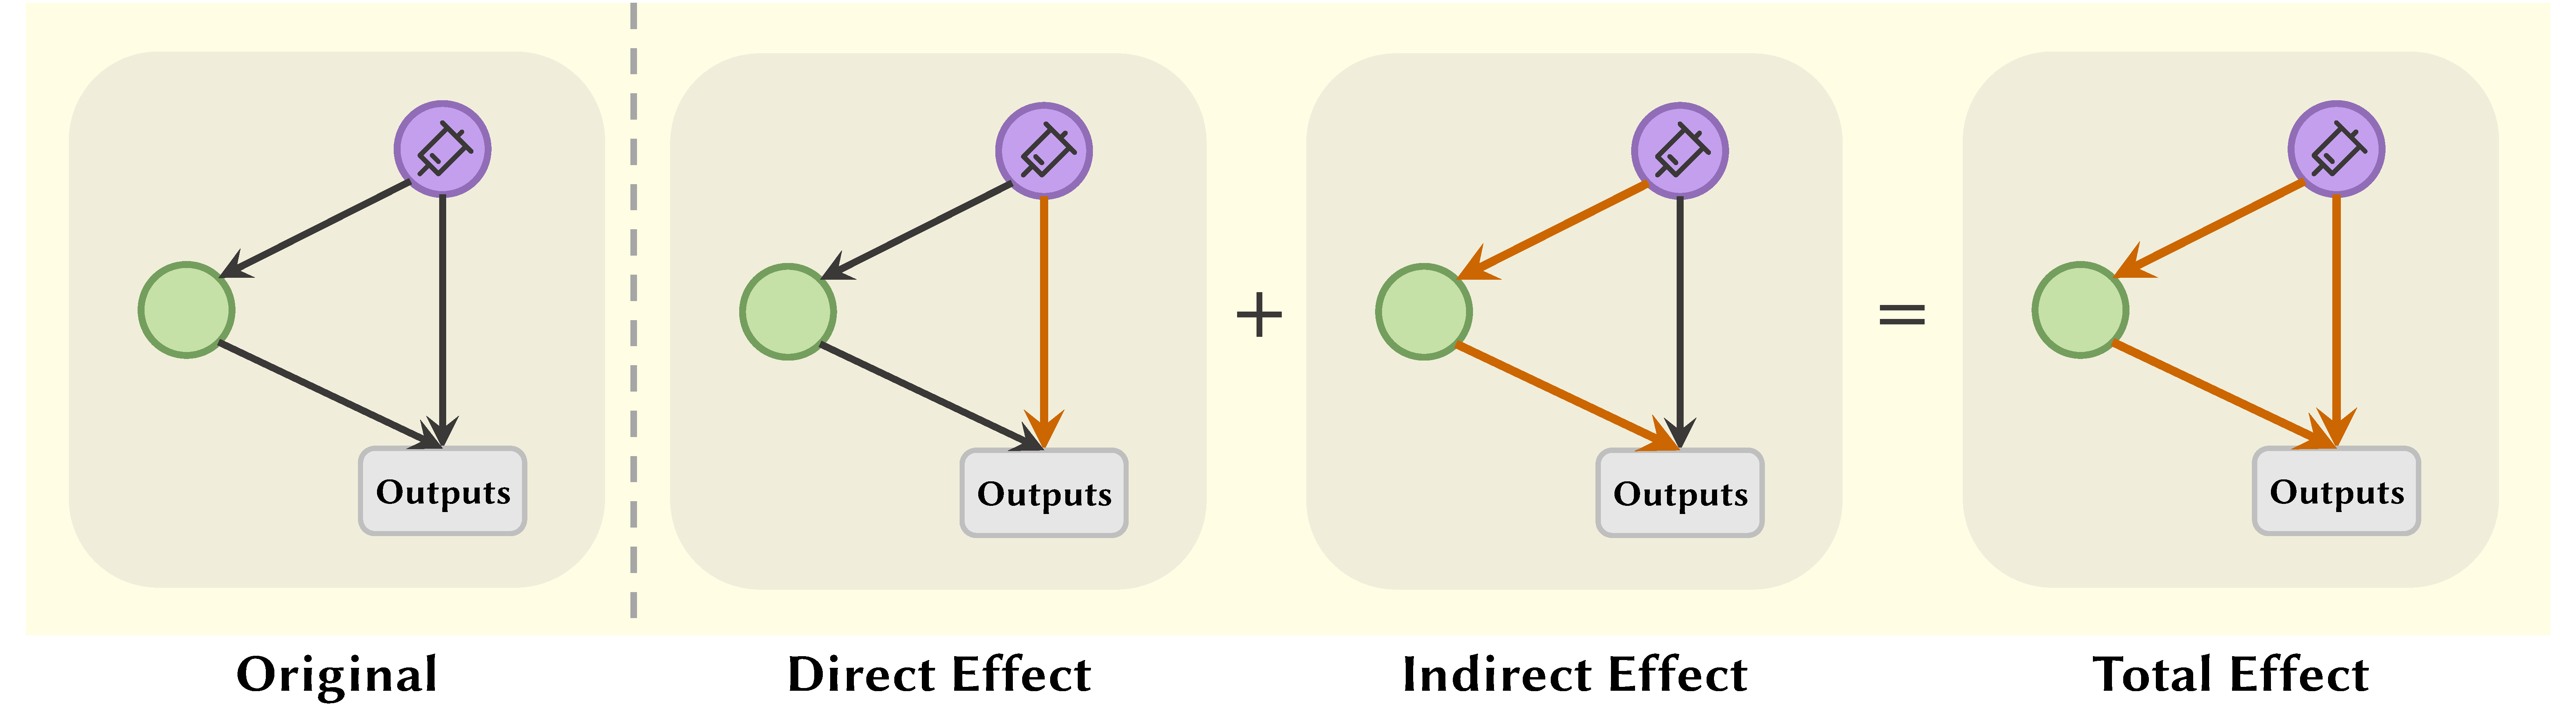
\includegraphics[width=0.85\linewidth]{figures/ThreeEffect.pdf}
    \caption{\revise{Three different types of calculating effects.}}
    \label{fig:ThreeEffect}
\end{figure}
\paragraph{\revise{Activation Patching}} \revise{Activation patching is aimed to analyze the impact of the modifications on the model's final decisions. It involves substituting activation values in specific layers of a model with alternatives—such as activations from different inputs, baseline values, or perturbed versions.} Specifically, three types of effects are considered: direct effect, indirect effect, and total effect, as illustrated in Figure~\ref{fig:ThreeEffect}.

\paragraph{\revise{Ablation study}} \revise{Ablation study and activation patching are conceptually related but differ in their methods of operation. Instead of replacing activations, it involves removing specific components of the LLM to observe how the output is affected.\citep{ActivationPatching_24_arXiv_Google} 
The key distinction between the two methods lies in their mechanism: activation patching modifies activations to simulate the logical replacement of a component, whereas ablation study physically removes the component entirely.}

\paragraph{Logit lens} When calculating effects like those shown in Figure~\ref{fig:ThreeEffect}, logit lens can quantify this effect. \revise{It is often used in conjunction with activation patching or ablation studies.} Specifically, it uses the unembedding layer to map an intermediate representation vector to the logits values of the vocabulary, allowing for the comparison of logits differences or other metrics. More details are in \href{https://colab.research.google.com/drive/1MjdfK2srcerLrAJDRaJQKO0sUiZ-hQtA}{the Colab notebook}.